%%%% SEITENRAENDER, SCHRIFTGROESSE UND ZEILENABSTAND NICHT ABAENDERN => SONST GIBT ES PUNKTEABZUG
\documentclass[a4paper,11pt,singlespacing]{article}
% \usepackage[left=2.5cm,right=2.5cm,top=2.5cm]{geometry}
\usepackage{setspace}
\usepackage[utf8]{inputenc}
\usepackage{graphicx}
\usepackage{color}
\usepackage{hyperref}
\usepackage{biblatex}
\usepackage[german]{babel}
\usepackage{tikz}
\usepackage{pgfplots}
\usepackage{float}
\usepackage{listings,xcolor}
\usepackage{caption}
\usepackage[acronym]{glossaries}
\makeglossaries
\addbibresource{sample.bib}

%opening
\title{Project title}
\author{
	Name Mat.No.
	}

\begin{document}
% Absatzeinrückung verhindern
\setlength{\parindent}{0ex}

\begin{titlepage}
	
	\newcommand{\HRule}{\rule{\linewidth}{0.5mm}} % Defines a new command for the horizontal lines, change thickness here
	
	\center % Center everything on the page
	
	%----------------------------------------------------------------------------------------
	%	HEADING SECTIONS
	%----------------------------------------------------------------------------------------
	
	\textsc{\LARGE University of Applied Sciences Ravensburg Weingarten}\\[1.5cm] % Name of your university/college
	\textsc{\Large Department of
		Electrical Engineering
		and Computer Science}\\[0.5cm] % Major heading such as course name
	\textsc{\large Bachelor Project}\\[0.5cm] % Minor heading such as course title
	
	%----------------------------------------------------------------------------------------
	%	TITLE SECTION
	%----------------------------------------------------------------------------------------
	
	\HRule \\[0.4cm]
	{ \huge \bfseries Patient Monitoring System}\\[0.4cm] % Title of your document
	\HRule \\[1.5cm]
	
	%----------------------------------------------------------------------------------------
	%	AUTHOR SECTION
	%----------------------------------------------------------------------------------------
	
	\begin{minipage}{0.4\textwidth}
		\begin{flushleft} \large
			\emph{Author:}\\
			Niklas \textsc{Kleiser}\\ % Your name
			Mat.No. 35579 \\
            Emircan \textsc{Tutar}\\ % Your name
			Mat.No. 35606 \\
            David \textsc{Metzler}\\ % Your name
			Mat.No. 35582
		\end{flushleft}
	\end{minipage}
	~
	\begin{minipage}{0.4\textwidth}
		\begin{flushright} \large
			\emph{Supervisor:} \\
			M.Sc. Benjamin \textsc{Stähle} % Supervisor's Name
		\end{flushright}
	\end{minipage}\\[2cm]
	
	% If you don't want a supervisor, uncomment the two lines below and remove the section above
	%\Large \emph{Author:}\\
	%John \textsc{Smith}\\[3cm] % Your name
	
	%----------------------------------------------------------------------------------------
	%	DATE SECTION
	%----------------------------------------------------------------------------------------
	
	{\large \today}\\[3cm] % Date, change the \today to a set date if you want to be precise
	
	%----------------------------------------------------------------------------------------
	%	LOGO SECTION
	%----------------------------------------------------------------------------------------
	
	
	
\includegraphics[width=7cm]{images/logo.png} % Include a department/university logo - this will require the graphicx package
	
	%----------------------------------------------------------------------------------------
	
	\vfill % Fill the rest of the page with whitespace
	
\end{titlepage}


\tableofcontents
\pagebreak

\section{Einleitung}

Im Zeitalter der Digitalisierung und des zunehmenden Einsatzes von kompakten Computermodulen wie dem Raspberry Pi in verschiedenen Anwendungsbereichen, steht die Entwicklung von robusten, skalierbaren und sicheren Systemen mehr denn je im Vordergrund. Dieses Dokument beschreibt ein Projekt, das darauf abzielt, ein Überwachungssystem für die Patientenpflege zu implementieren, wobei der Schwerpunkt auf der Nutzung verschiedener Technologien und Frameworks liegt, um eine effiziente und effektive Lösung zu gewährleisten.

Das Projekt nutzt die Stärken von Docker, um eine isolierte und konsistente Umgebung für die Ausführung verschiedener Dienste auf einem einzigen Raspberry Pi zu schaffen. Dies ist von entscheidender Bedeutung, da es die Wartung und Skalierung des Systems vereinfacht und gleichzeitig die Sicherheit durch die Isolation der einzelnen Anwendungen erhöht. Darüber hinaus stellt die Verwendung von Ubuntu 22.04 LTS eine stabile und unterstützte Basis dar, die die Langlebigkeit und Zuverlässigkeit des Systems sicherstellt.

Die Implementierung dynamischer DNS-Management-Dienste, spezifischer Sicherheitsmechanismen wie Fail2Ban und die Integration fortschrittlicher Kommunikationstechnologien wie MQTT zeigen die Vielseitigkeit und Anpassungsfähigkeit des entwickelten Systems. Zusätzlich zur Kernfunktionalität, die durch die technische Implementierung erreicht wird, umfasst dieses Projekt auch die Erstellung einer angepassten Firewall, die Einrichtung eines Mail-Servers und die Verwendung von Matrix für eine nahtlose und sichere Kommunikation.

Mit diesem Projekt treiben wir nicht nur die technische Entwicklung voran, sondern setzen auch neue Maßstäbe in der Patientenüberwachung. Es zeigt, wie durch den Einsatz moderner Technologien die Lebensqualität von Menschen verbessert und die Arbeit von medizinischem Personal unterstützt werden kann. Die dokumentierten Abschnitte bieten eine detaillierte Darstellung der technischen Anforderungen, der Architektur sowie der tatsächlichen Implementierung des Systems und motiviert alle Beteiligten, auf diesen Grundlagen weiter aufzubauen und die Technologie zum Wohl der Gesellschaft einzusetzen.
\selectlanguage{german}

\section{Grundbegriffe}

\subsection{Docker}
Docker ist eine Open-Source-Softwareplattform, die die Virtualisierung auf Betriebssystemebene nutzt, um Software in Paketen, sogenannten Containern, zu entwickeln, auszuliefern und auszuführen. Container ermöglichen es, eine Anwendung mit allen Teilen, die sie zum Ausführen benötigt, wie Bibliotheken und andere Abhängigkeiten, zu kapseln und auf jedem Linux-System auszuführen, als wären sie auf einem dedizierten Computer installiert. Dies gewährleistet die Konsistenz unabhängig von der Umgebung und verbessert die Sicherheit, da Anwendungen isoliert voneinander ausgeführt werden.

\subsection{MQTT (Message Queuing Telemetry Transport)}
MQTT ist ein Netzwerkprotokoll, das speziell für die Bedürfnisse von Internet-of-Things (IoT)-Anwendungen entwickelt wurde. Es ermöglicht es Geräten, Daten in einem schwach vernetzten Netzwerk effizient zu übertragen. Das Protokoll basiert auf einem Publisher/Subscriber-Modell, das eine hohe Nachrichtenübermittlungseffizienz bei gleichzeitig geringem Ressourcenbedarf bietet. MQTT wird häufig in der Heimautomatisierung, in der Medizintechnik und anderen Bereichen verwendet, in denen eine zuverlässige und effiziente Kommunikation zwischen einer Vielzahl von Geräten erforderlich ist.

\subsection{Raspberry Pi}
Der Raspberry Pi ist ein kleiner, preiswerter Einplatinencomputer, der ursprünglich für Bildungszwecke entwickelt wurde, aber aufgrund seiner Vielseitigkeit und Leistungsfähigkeit in einer Vielzahl von industriellen und Hobby-Projekten eingesetzt wird. Der Pi kann mit verschiedenen Betriebssystemen wie Raspbian, einem Debian-basierten Linux, betrieben werden und unterstützt eine breite Palette von Anwendungen und Programmiersprachen.

\subsection{Fail2Ban}
Fail2Ban ist eine Intrusion Prevention Software, die durch Überwachen von Serverprotokollen auf Muster von Missbrauchsversuchen wie zu viele fehlgeschlagene Anmeldeversuche reagiert. Wenn ein solches Muster erkannt wird, konfiguriert Fail2Ban die Firewall des Hosts temporär so, dass sie IP-Adressen blockiert, von denen aus die verdächtigen Aktivitäten ausgehen, um so das System zu schützen.

\subsection{Ubuntu 22.04 LTS}
Ubuntu 22.04 LTS ist eine Version des Ubuntu-Betriebssystems, die auf Stabilität und langfristige Unterstützung ausgerichtet ist, was sie besonders für Unternehmensumgebungen geeignet macht. Es bietet regelmäßige Sicherheitsupdates für fünf Jahre, was eine zuverlässige Grundlage für Projekte gewährleistet, die eine langfristige Wartbarkeit erfordern.

\subsection{DDclient}
DDclient ist ein Perl-Script, das zur automatischen Aktualisierung von DNS-Einträgen genutzt wird, um dynamisch zugewiesene IP-Adressen mit einem festen Hostnamen zu verknüpfen. Dies ist besonders nützlich in Umgebungen mit dynamischer IP-Zuweisung, wie sie bei vielen Internetdienstanbietern üblich ist.

\subsection{SMTP-Server}
Ein Simple Mail Transfer Protocol (SMTP)-Server ist ein Netzwerkserver, der E-Mails sendet und empfängt. Er spielt eine zentrale Rolle in der elektronischen Kommunikation und wird häufig in Unternehmensumgebungen eingesetzt, um die interne und externe Kommunikation zu verwalten.

\subsection{Matrix}
Matrix ist ein offenes Protokoll für Echtzeitkommunikation, das speziell für die Anforderungen des modernen Internets entwickelt wurde. Es unterstützt verschlüsselte Chat-, VoIP- und Videokonferenzdienste und ermöglicht die Interoperabilität über verschiedene Kommunikationsplattformen hinweg.


\selectlanguage{german}

\section{Lastenheft}
\begin{itemize}
    \item Sicherheitsaspekt
    \item Funktional 
    \item Interaktionsschnitstelle
\end{itemize}

\subsection{Muss - Anforderungen}
\begin{itemize}
  \item ddclient
  \item Alarm Ton
  \item Ubuntu 22.04 (LTS, Sec)
  \item Docker / Docker Compose
\end{itemize}

\subsection{Fail2ban}
Fail2Ban ist ein entscheidendes Werkzeug zur Absicherung, die dazu dient, einen Server vor unautorisierten Zugriffsversuchen und Brute-Force-Angriffen zu schützen. Durch die Überwachung von Logdateien erkennt Fail2Ban auffällige Anmeldeversuche und blockiert die zugehörigen IP-Adressen automatisch für eine vordefinierte Zeitdauer. Mit Fail2Ban kann beispielsweise die IP-Adresse eines Geräts, das wiederholt versucht, ohne die korrekten Anmeldedaten eine Verbindung zum Server herzustellen, blockiert werden. Es lässt sich so konfigurieren, dass jede IP-Adresse, die mehr als dreimal pro Tag versucht, sich zu verbinden, gesperrt wird. \cite{Fail2ban} Diese Funktion ist besonders wichtig für die Minimierung von potenziellen Sicherheitsrisiken. Im Rahmen unseres Projekts auf dem Raspberry Pi wird Fail2Ban eine kritische Rolle spielen, indem es dazu beiträgt, die Zugriffskontrolle auf unsere Dienste wie SSH verstärken.

\subsection{MQTT / MQTT-Client}
Unser System wird aus mehreren verschiedenen Komponenten bestehen, die miteinander kommunizieren müssen. Diese Kommunikation muss über einen Message - Broker und das Protokoll ''MQTT'' erfolgen \cite{MQTT} . Um das Protokoll nutzen zu können benötigt es einen MQTT - Message Broker und Clients die ihre Nachrichten an diesen schicken, dass sie an die Clients verteilt werden, die darum gebeten haben Nachrichten eines Topics zu erhalten. 

\subsection{SMTP-Server / SMTP-Client}
Zu Zwecken der Protokollierung und Dokumentation muss das System zusätzlich zu einem Alarm eine Mail an einen eigenen Mailserver gesendet werden. Dieser Mailserver soll über das SMTP - Protokoll Mails empfangen können. Es muss somit ein Mailcow - Server eingerichtet werden  \cite{Mailcow} . Dafür müssen auch DNS - Records angepasst werden. 

\subsubsection{Raspberry und Raspberry Pi} \label{sec:raspi}
Für das Projekt soll der Raspberry Pi gewählt werden, da dieser eine einfache Anbindung mit einer Kamera erlaubt \cite{Raspberry}  \cite{Raspberry_camera}. Der Raspberry Pi erlaubt es Microcontroller und Kamera in einem kompakten Gehäuse unterzubringen.  Es soll zwei Raspberry Pis geben, die eine Detektion  durchführen (siehe Abb. \ref{fig:patient_monitoring}). Ein Raspberry Pi mit Raspberry Pi Kamera übernimmt die Bed Detektion und ein Raspberry Pi mit Kamera übernimmt die Fall Detektion. Ein dritter Raspberry Pi soll  dafür verwendet werden,  einen Alarm zu schalten. 

\begin{figure}[H]
	\hspace{-0.5cm}
	\begin{tikzpicture}
		
	
		\draw [-, dashed, gray] (4,1)-- (-4,1)--(-4,3.5) --(4,3.5) --(4,1);
		
			\node at (-2.8 ,3) {BED VIEW};
					
		\node[inner sep=0pt] (whitehead) at (2,2.5)
		{
\includegraphics[width=.05\textwidth]{images/camera.png}};
		
		\node[above] at (2.2,2.6) {\scriptsize Raspberry Pi und Kamera};
		
		\node[inner sep=0pt] (whitehead) at (0,2)
		{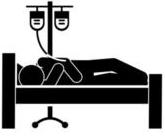
\includegraphics[width=.1\textwidth]{images/person_in_bed.png}};

			\node at (-2.6 ,-1) {ROOM VIEW};
	
			\draw [-, dashed, gray] (4,-0.5)-- (-4,-0.5)--(-4,-4) --(4, -4 ) --(4,-0.5);
		
		\node[inner sep=0pt] (whitehead) at (2,-1.5)
		{
\includegraphics[width=.05\textwidth]{images/camera.png}};
		

		
		\node[inner sep=0pt] (whitehead) at (-0.25,-1.25)
		{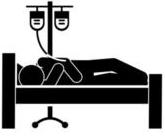
\includegraphics[width=.1\textwidth]{images/person_in_bed.png}};
		
		
		\node[inner sep=0pt] (whitehead) at (0,-2.25)
		{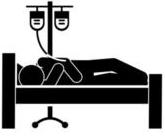
\includegraphics[width=.1\textwidth]{images/person_in_bed.png}};
		
	\node[inner sep=0pt] (whitehead) at (-0.5,-3.25)
		{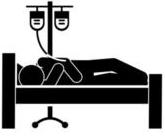
\includegraphics[width=.1\textwidth]{images/person_in_bed.png}};
		

	  \node[inner sep=0pt] (whitehead) at (4.0,0.25)
		{
\includegraphics[width=.08\textwidth]{images/server.png}};
		
				\node[below] at (2.2,-1.6) {\scriptsize Raspberry Pi und Kamera};
		
		\node[below] at (4.0,-0.1) {\scriptsize MQTT Broker};
		
			
		
		\draw [-] (2,2.5)-- ( 3,2.5) -- (3,0.25) ;
		\draw [-] (2,-1.5)-- ( 3,-1.5) -- (3,0.25) ;
		\draw [-]  (3,0.25)  -- (3.8,0.25);

	    \draw [->]  (4.2 ,0.25) -- (5.0,0.25) -- (5.0,-1.5) -- (5.5,-1.5);
	     \draw [->]  (4.2 ,0.25) -- (5.0,0.25) -- (5.0,2.5) -- (5.5,2.5);
	
		\node at  (7.0,2.5) {Bed Detection};
		
		
		\node at  (7.0,-1.5) {Fall Detection};
		
		
	
	 	\draw [->]  (8.5 ,-1.5) -- (9.0,-1.5) -- (9,0.25) -- (9.5,0.25)  ;
	
		\draw [->]  (8.5, 2.5) -- (9.0,2.5) -- (9,0.25) -- (9.5,0.25) ;
		
		\node[inner sep=0pt] (whitehead) at (9.85,0.25)
		{
\includegraphics[width=.05\textwidth]{images/raspi.png}};
		
		\node[below] at (10.,0.1) {\scriptsize Raspberry Pi };
		
		\draw [->]  (10.3,0.25) -- (10.6,0.25) ;
		
		\node[red] at  (11.2,0.25) {Alarm};
		
		
	\end{tikzpicture}
	\caption{Darstellung des Systemaufbaus}
	\label{fig:patient_monitoring}
\end{figure}


\subsubsection{Fall Detektion}
In Abschnitt  \ref{sec:raspi} wurde bereits angerissen, dass ein Raspberry Pi mithilfe der Raspberry Pi Kamera eine Fall Detektion durchführen soll. Der Raspberry Pi soll also überprüfen, ob ein Patient hingefallen ist. Dies soll mithilfe des Yolo-Frameworks gemacht werden \cite{Yolo}. Es ist hierbei Ziel das Modell auf dem Raspberry Pi zum Laufen zu bekommen, um möglichst nicht noch einen zusätzlichen Server zu benötigen. 

\subsubsection{Matrix}
Es soll einen Matrixserver geben \cite{Matrix} . Über diesen Server sollen Pfleger auch auf dem Handy benachrichtigt werden, wenn eine Alarmsituation eingetreten ist. 


\subsection{Soll - Anforderungen}
\begin{itemize}
  \item Self-Hosted
  \item Alarm Licht
  \item Firewall (Router hat ja eh ne Firewall)
\end{itemize}

\subsubsection{Bett Detektion}
Es soll eine Komponente in unserem System geben, welche sich darum kümmert, zu erkennen, ob eine Person in einem Bett liegt. Es soll aber nicht jede Abwesenheit sofort zu einem Alarm führen, sondern nur, wenn über einen Zeitraum von 10 Minuten, das Bett leer bleibt, sollte ein Pfleger benachrichtigt werden, der dann nach dem Patienten schaut. Aufgrund der Zeitspanne von 10 Minuten, die das Bett leer bleiben muss, um einen Alarm auszulösen, ist es auch in Ordnung, wenn die Detektion etwas länger dauert. Es soll angestrebt werden, innerhalb von 30 Sekunden nach Verlassen des Betts zu erkennen das dieses leer ist. 

\subsection{Kann - Anforderungen}

\subsection{MQTT Frontend}
Es kann ein MQTT - Frontend benutzt werden, um es Entwicklern einfacher zu machen die verschiedenen Nachrichten und Kommunikationskanäle nachzuvollziehen. 

\subsection{Gesprochene Information über Patient in Hilfesituation}
In den Minimalanforderungen unseres Systems weiß ein Pfleger nur das ein Patient Hilfe benötigt, nicht aber, welcher der Patienten. Um diese Problematik zu lösen, kann das System anstelle des Alarmtons über eine sprechende Stimme dem Pfleger mitteilen, welcher Patient Hilfe benötigt. 

\subsubsection{Kameraview}
Falls noch Zeit ist, soll zusätzlich mithilfe des QT-Frameworks eine Kameraview  in Python entwickelt werden \cite{Python} \cite{QT} . Mit dieser Anwendung sollen  Pfleger die Patienten überwachen können. Sie können so Dinge entdecken, die durch unsere Detektoren nicht abgedeckt werden. Ein Pfleger könnte so die Extubation eines Patienten erkennen. 

\selectlanguage{german}
\clearpage

\section{Kommunikation}

\selectlanguage{german}

\subsection{Einführung in MQTT}
MQTT (Message Queuing Telemetry Transport) ist ein leichtgewichtiges Protokoll, das speziell für die Kommunikation zwischen Geräten mit begrenzten Ressourcen entwickelt wird. Es zeichnet sich durch seine Effizienz und geringe Bandbreitennutzung aus, was es ideal für den Einsatz in IoT (Internet of Things) und anderen Umgebungen mit eingeschränkten Netzwerkressourcen macht.

\subsection{MQTT - Architektur}
MQTT arbeitet nach einem Publisher/Subscriber-Modell, bei dem Clients Nachrichten zu bestimmten Themen ("Topics") veröffentlichen oder abonnieren. Ein zentraler Broker verwaltet diese Kommunikation, indem er die Nachrichten vom Publisher an die abonnierten Subscriber weiterleitet. Es muss gewährleistet sein, dass dieser Broker funktioniert und erreichbar ist, da ohne ihn keine Kommunikation zwischen Subscriber und Publisher möglich ist.

\subsection{Sicherheitsaspekt}
Authentifizierung stellt sicher, dass nur autorisierte Geräte Zugang zum Broker erhalten. Der Message-Broker erlaubt nur Kommunikation mit authentifizierten Publishern und Subscribern. Nicht authentifizierte Clients werden abgelehnt. Die Verschlüsselung der Kommunikation zwischen Clients und dem Broker erfolgt über TLS (Transport Layer Security). Dies schützt die Daten vor Abhören und Manipulation durch Dritte.

\subsection{Setup des Message-Brokers}
Um über das MQTT-Protokoll zu kommunizieren, ist der erste Schritt die Installation und Konfiguration eines MQTT-Brokers. Bekannte MQTT-Broker sind Mosquitto und HiveMQ. Der Eclipse-Mosquitto-Docker-Container wird verwendet. Der Message-Broker wird nun über die mosquitto.conf konfiguriert, sodass nur authentifizierte Clients mit dem Broker kommunizieren dürfen. Ein Account wird erstellt, dessen Zugangsdaten Clients zur Authentifizierung am Broker verwenden müssen.

\subsection{Integration mit anderen Komponenten}
Die Integration mit anderen Komponenten des Systems ist einfach, da MQTT ein weitverbreitetes Protokoll ist und in vielen Sprachen Implementationen eines MQTT-Clients existieren. Über diesen können Nachrichten an den Message-Broker und somit an andere Clients gesendet werden. Es muss nur noch festgelegt werden, wie die Nachrichten aussehen. Da die Nachrichtenformate den speziellen Bedingungen und Anforderungen der Kommunikationspartner unterliegen, wird nicht darauf festgelegt, dass dieselben Nachrichten-Inhalte im ganzen System gleich aussehen.


\selectlanguage{german}

\section{Implementierung}

\selectlanguage{german}
\subsection{YOLOv5}
\nameref{subsec:yolo}, ein Bilderkennungsmodell, wurde von Joseph Redmon und Ali Farhadi an der Universität von Washington entwickelt und im Jahr 2015 veröffentlicht. \nameref{subsec:yolo} steht für "You Only Look Once", was darauf hinweist, dass das Modell nur einmal auf ein Bild schaut, um Objekte schnell und präzise zu erkennen. Seit seiner Veröffentlichung wurden insgesamt neun Versionen von \nameref{subsec:yolo} veröffentlicht \cite{Yolo} .

\subsubsection{Das Modell}
Ein vortrainiertes Modell der fünften Version von \nameref{subsec:yolo} wird verwendet, welches bereits spezifisch für die gegebenen Anforderungen trainiert ist. Obwohl es sich um eine ältere Version von YOLOv5 handelt, ist die Effektivität des Modells nicht beeinträchtigt. YOLOv5 zeigt gerade bei begrenzten Hardware-Ressourcen wie dem Raspberry Pi 4 eine höhere Geschwindigkeit im Vergleich zu neueren Versionen wie YOLOv8. Vorteilhaft ist auch, dass eine kleinere Variante von \nameref{subsec:yolo}, nämlich Yolov5s, genutzt wird. Dieses Modell wurde mit Bildern aus diversen Quellen trainiert, wobei ein benutzerdefiniertes Datenset aus 374 Trainingsbildern und 111 Validierungsbildern erstellt wurde.

\subsubsection{Makesense.ai}
Für das Labeln der Daten kommt Makesense.ai zum Einsatz, eine Plattform, die es Nutzern erlaubt, Bilder hochzuladen und mit Annotationen wie Bounding Boxes und Klassifizierungen zu versehen. Dies dient der Vorbereitung von Datensätzen für Anwendungen in der Computer Vision \cite{noauthor_make_nodate}. Die Daten sind dabei in drei Klassen untergliedert: 'walking', 'sitting' und 'fall detected' (siehe Abbildung \ref{fig:yolo_classes}).


\begin{figure}[H]
	\centering
	\begin{minipage}[b]{0.3\textwidth}
		\centering
		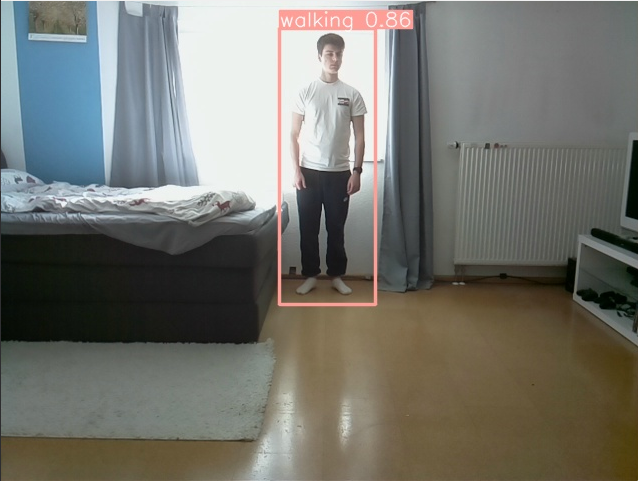
\includegraphics[width=\textwidth]{images/walking.png}
		\caption*{Klasse: ''walking''}
	\end{minipage}
	\hfill
	\begin{minipage}[b]{0.3\textwidth}
		\centering
		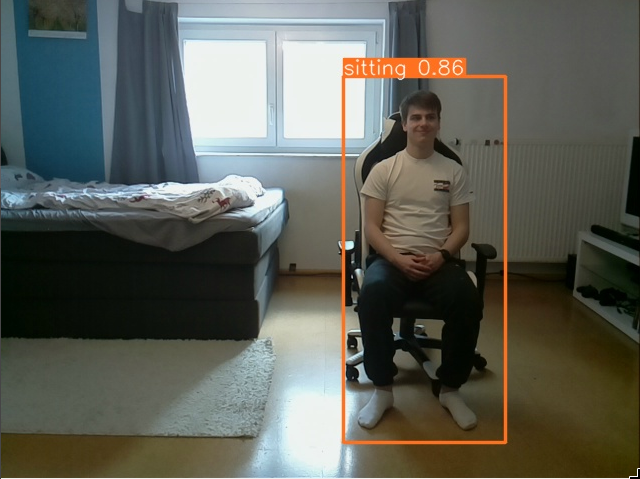
\includegraphics[width=\textwidth]{images/sitting.png}
		\caption*{Klasse: ''sitting''}
	\end{minipage}
	\hfill
	\begin{minipage}[b]{0.3\textwidth}
		\centering
		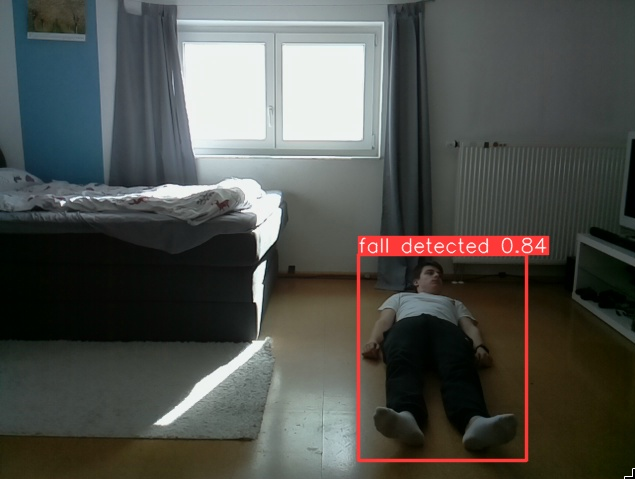
\includegraphics[width=\textwidth]{images/fallen.png}
		\caption*{Klasse: ''fall detected''}
	\end{minipage}
	\caption{YOLOv5 Detektion Klassen}
	\label{fig:yolo_classes}
\end{figure}



\subsubsection{Anbindung}
Die Anbindung an das YOLOv5-Modell erfolgt über PyTorch, ein Open-Source-Framework für maschinelles Lernen, das auf der Programmiersprache Python und der Torch-Bibliothek basiert. PyTorch wurde 2016 von einem Forscherteam für künstliche Intelligenz bei Facebook entwickelt \cite{noauthor_pytorch_nodate}.

Das Modell läuft in einem Docker-\nameref{subsec:container}, der kontinuierlich über MQTT einen boolean-Wert veröffentlicht, um anzuzeigen, ob ein \nameref{subsec:alarm} aufgetreten ist. Zur Einbindung der Raspberry Pi Kamera verwendet der \nameref{subsec:container} auch OpenCV, eine Open-Source-Bibliothek für Computer Vision \cite{OpenCV}. Mithilfe von OpenCV wird auch eine Funktion entwickelt, die über \nameref{subsec:mqtt} ein Bild mit allen Detektionen versendet. Diese Bilder werden später mithilfe eines weiteren \nameref{subsec:docker} Containers auf einem lokalen Rechner angezeigt.

\subsubsection{Evaluation}
Das Modell soll dem Model-Entwickler zufolge eine Genauigkeit von 85 bis 90\% bei Tageslicht haben. Es hat jedoch Schwierigkeiten mit der Detektion von vielen Personen auf einem Bild, was zu falschen Erkennungen führen kann. Für diesen Anwendungsfall, d.h. die Überwachung von Patienten, ist dies jedoch kein Problem, da es in den Bildern normalerweise nur einzelne Patienten gibt. 

% Zitat von wo das 85% bis 90% genauigkeit ist. Quelle fehlt, noch ergänzen.


\clearpage

\selectlanguage{german}
\subsection{Matrix}

\nameref{subsec:matrix} ist einen offener Standard für interoperable, dezentrale, Echtzeitkommunikation über das Internetprotokoll (IP). Nutzer verbinden sich mit einem Heim-Server und können Räume auf jedem Matrix-Server betreten, was die Kommunikation über Servergrenzen hinweg ermöglicht. Nachrichten werden zwischen den Servern synchronisiert, was eine unterbrechungsfreie Kommunikation sicherstellt, auch wenn ein Server offline geht. \nameref{subsec:matrix} unterstützt Ende-zu-Ende-Verschlüsselung für sichere Gespräche. Zur Erprobung von \nameref{subsec:matrix} lassen sich zahlreiche Matrix-Clients verwenden \cite{noauthor_introduction_nodate}. Ein \nameref{subsec:docker} Container wird eingesetzt, um den Matrix Home-Server zu hosten \cite{noauthor_matrixdotorgsynapse_nodate}. Matrix dient dazu, Pfleger mittels eines \nameref{subsec:alarm} zu informieren.

\subsubsection{Element}
Der Matrix-Client Element wird für die Kommunikation genutzt \cite{noauthor_element_nodate}. Element, geleitet von den Entwicklern von \nameref{subsec:matrix}, bietet eine benutzerfreundliche Oberfläche sowie zahlreiche Funktionen, die den spezifischen Anforderungen entsprechen.

\subsubsection{Nginx reverse proxy}

Ein \nameref{subsec:reverseproxy} wird benötigt, damit der Matrix-Server auch \nameref{subsec:ssl} nutzen kann. Ein \nameref{subsec:reverseproxy} agiert als Vermittler zwischen Clients, wie beispielsweise Webbrowsern, und Webservern. Anstelle einer direkten Kommunikation mit dem Ursprungsserver senden Clients ihre Anfragen an den \nameref{subsec:reverseproxy}, der diese an den zuständigen Server weiterleitet und die Antworten an die Clients zurücksendet \cite{noauthor_was_nodate}. Nginx wird als \nameref{subsec:reverseproxy} verwendet \cite{noauthor_nginx_nodate}, da dieser Server umfassend dokumentiert und weit verbreitet ist. Nginx ist als \nameref{subsec:docker}-Container verfügbar, was die Integration erleichtert \cite{noauthor_nginx_nodate}.


\begin{figure}[H]
\begin{tikzpicture}[scale=0.7]
	
		\node[inner sep=0pt] (whitehead) at (-10,2)
	{
\includegraphics[width=0.15\textwidth]{images/computer.png}};
	
	\node[font=\scriptsize] at (-10,1.2) {\scriptsize Laptop 1} ;
	
	\draw[->] (-9.2,1.8)--(-6.5,0.5) node[pos=0.5, above,rotate=-28] { \scriptsize example.org};
	
		\node[inner sep=0pt] (whitehead) at (-10,0)
	{
\includegraphics[width=0.15\textwidth]{images/computer.png}};
	
		\node[font=\scriptsize] at (-10,-0.8) {\scriptsize Laptop 2};
	
		\draw[->] (-9,0)--(-6.5,0) node[pos=0.45, above] { \scriptsize example.org};
	
		\node[inner sep=0pt] (whitehead) at (-10,-2)
	{
\includegraphics[width=0.15\textwidth]{images/computer.png}};
	
			\node[font=\scriptsize] at (-10,-2.8) {\scriptsize Laptop 3};
	
		\draw[->] (-9.2,-1.8)--(-6.5,-0.5)  node[pos=0.5, above,rotate=28] { \scriptsize example.org};
	
		\node[inner sep=0pt] (whitehead) at (-5,0)
	{
\includegraphics[width=0.10\textwidth]{images/cloud.png}};
	
				\node[font=\scriptsize] at (-5,-0.8) {\scriptsize Internet};
	
		\draw[->] (-4,0)--(-1,-0);
	
	\node[inner sep=0pt] (whitehead) at (0,0)
	{
\includegraphics[width=0.10\textwidth]{images/switch.png}};
	
		\node[font=\scriptsize] at (0,-0.8) {\scriptsize reverse proxy};
	
	\draw[->] (1,0.2)--(4,0.8);
	
		\draw[->] (1,-0.2)--(4,-0.8);
	
		\node[inner sep=0pt] (whitehead) at (5,1)
	{
\includegraphics[width=0.10\textwidth]{images/switch.png}};
	
			\node[font=\scriptsize] at (5,0.4) {\scriptsize matrix server};
	
			\node[inner sep=0pt] (whitehead) at (5,-1)
	{
\includegraphics[width=0.10\textwidth]{images/switch.png}};
	
		\node[font=\scriptsize] at (5,-1.6) {\scriptsize mail server};
	
\end{tikzpicture}
	\caption{Aufbau eiens reverse proxies}
\label{fig:patient_reverse_proxy}
\end{figure}

\subsubsection{Postgres}
Die Einrichtung des \nameref{subsec:matrix} Docker-Containers mit PostgreSQL wird empfohlen (siehe \cite{noauthor_installation_nodate}). Standardmäßig dient SQLite als Datenbank, da es die Konfiguration vereinfacht. Für eine verbesserte Leistungsoptimierung empfiehlt es sich jedoch, PostgreSQL zu verwenden, das besser optimiert ist. PostgreSQL ist ein leistungsstarkes Datenbanksystem, das SQL verwendet und erweitert. Es bietet zahlreiche Funktionen zur sicheren Speicherung und Skalierung komplexer Datenlasten und wurde im Rahmen des POSTGRES-Projekts an der University of California in Berkeley entwickelt \cite{noauthor_postgresql_nodate}.

\subsubsection{Certbot}
Um die Unterstützung der \nameref{subsec:ssl}-Verschlüsselung auf dem Matrixserver sicherzustellen, ist ein \nameref{subsec:sslcertificate} notwendig. \nameref{subsec:ssl} (Secure Sockets Layer) sichert Internetverbindungen durch Verschlüsselung der Daten zwischen Browsern und Servern und gewährleistet die Vertraulichkeit sowie Integrität sensibler Informationen. Zudem ermöglicht es die Authentifizierung des Servers gegenüber dem Browser, um sicherzustellen, dass die Verbindung authentisch und sicher ist \cite{SSL}. Certbot ist ein benutzerfreundlicher Client, der ein Zertifikat von Let's Encrypt abruft.  Das \nameref{subsec:sslcertificate} von Let's Encrypt ist kostenlos. 

\subsubsection{Matrix Bridge}
Eine Matrix-Bridge wird verwendet, um den E-Mail-Server mit \nameref{subsec:matrix} zu verbinden \cite{jojii_jojiiofficialmatrix-emailbridge_2024}. Bridges in Matrix erleichtern die Verbindung zu anderen Plattformen und unterstützen die Interoperabilität, was die Vernetzung von Matrix über verschiedene digitale Plattformen hinweg ermöglicht \cite{noauthor_bridges_nodate}. Die Bridge gestattet es, E-Mails über Matrix zu senden und E-Mail-Inhalte in Matrix verfügbar zu machen. Alarme werden mit der Bridge, ausschließlich über E-Mail ausgelöst, die automatisch auch nach Matrix versendet wird.


\subsubsection{Matrix Client}
Eine eigenständige Matrix-Clientanwendung wurde als zusätzliche Sicherheitsmaßnahme entwickelt, um im Falle eines Ausfalls des E-Mail-Servers Nachrichten zu versenden. Sie ist direkt mit der Matrix-Bridge integriert und wurde unter Einsatz der Nio-Bibliothek für die Matrix-API entwickelt \cite{nio}. Diese Anwendung sendet automatisch eine Benachrichtigung, sobald über MQTT gemeldet wird, dass eine Person gestürzt ist.

\clearpage

\selectlanguage{german}
\subsection{Mailcow}

\subsubsection{Einführung in Mailcow}
Mailcow ist eine Open-Source-Mailserver-Suite, die eine umfassende E-Mail-Lösung bietet. Verschiedene Dienste wie Postfix für den Mail-Transport, Dovecot für die Speicherung und den Zugriff auf E-Mails sowie SOGo als Webmail-Oberfläche werden kombiniert. Eine benutzerfreundliche Weboberfläche ermöglicht die Verwaltung von Domains, Benutzern und E-Mail-Quotas. Durch die Integration von modernen Sicherheitsmechanismen wie DMARC, DKIM und SPF wird ein hohes Maß an Sicherheit für die E-Mail-Kommunikation gewährleistet.

\subsubsection{IMAP / SMTP}
IMAP (Internet Message Access Protocol) und SMTP (Simple Mail Transfer Protocol) sind grundlegende Protokolle für den E-Mail-Verkehr. IMAP wird verwendet, um E-Mails vom Server zu lesen und zu verwalten, während SMTP zum Versenden von E-Mails dient. In Mailcow übernimmt Dovecot die Rolle des IMAP-Servers und Postfix die des SMTP-Servers.

\subsubsection{DNS MX-Record}
Der DNS MX-Record (Mail Exchanger Record) ist ein entscheidender Teil der E-Mail-Infrastruktur. Dieser Record gibt an, welche Mailserver für den Empfang von E-Mails für eine bestimmte Domain verantwortlich sind. Bei der Konfiguration von Mailcow muss der MX-Record der Domain auf den Mailcow-Server zeigen, um sicherzustellen, dass eingehende E-Mails korrekt zugestellt werden. Eine richtige Konfiguration des MX-Records ist notwendig für die Zustellung von E-Mails. Da die richtige Konfiguration des DNS notwendig ist, hat das Mailcow - Dockerized Projekt in ihrer Dokumentation Beschreibungen, wie man diesen richtig aufsetzt \cite{mailcowDockerizedDNS}.

\subsubsection{Sicherheit: DKIM}
DKIM (DomainKeys Identified Mail) ist ein Authentifizierungsprotokoll, das E-Mails mit einer digitalen Signatur versieht. Diese Signatur wird von einem öffentlichen Schlüssel überprüft, der im DNS der sendenden Domain veröffentlicht ist \cite{dkim}. DKIM hilft sicherzustellen, dass E-Mails nicht verändert wurden und wirklich von der angegebenen Domain stammen. In Mailcow kann ein DKIM-Schlüssel-Paar leicht über die Weboberfläche erstellt werden, um die Authentizität der ausgehenden E-Mails zu gewährleisten. Der öffentliche Schlüssel muss dann noch in einem DNS Record eingetragen werden.

\subsubsection{Sicherheit: SPF}
SPF (Sender Policy Framework) Mail Records sind ein Mechanismus zur Verhinderung von E-Mail-Spoofing. Sie ermöglichen es einem Domaininhaber, festzulegen, welche Mail-Server berechtigt sind, E-Mails im Namen ihrer Domain zu senden \cite{spf_erklärung}. Dies wird durch die Veröffentlichung eines SPF-Eintrags im DNS der Domain erreicht, der eine Liste autorisierter IP-Adressen enthält. E-Mail-Empfangsserver überprüfen den SPF-Eintrag der absendenden Domain und verwerfen oder markieren E-Mails als Spam, wenn sie von einem nicht autorisierten Server gesendet wurden. Dadurch wird die Wahrscheinlichkeit reduziert, dass schädliche oder gefälschte E-Mails erfolgreich zugestellt werden.

\subsubsection{Sicherheit: DMARC}
DMARC (Domain-based Message Authentication, Reporting, and Conformance) Mail Records bauen auf den Mechanismen von SPF und DKIM auf, um eine umfassendere E-Mail-Authentifizierung zu bieten. DMARC ermöglicht es, Richtlinien zu definieren, wie E-Mail-Empfangsserver mit Nachrichten umgehen sollen, die SPF- oder DKIM-Prüfungen nicht bestehen \cite{dmarc_erklärung}. Ein DMARC-Eintrag im DNS der Domain legt fest, ob solche E-Mails abgewiesen, in Quarantäne gestellt oder zugestellt werden sollen, und bietet zudem eine Reporting-Funktion. Dadurch können Domaininhaber Berichte über gefälschte E-Mails erhalten und ihre E-Mail-Sicherheitsrichtlinien kontinuierlich verbessern. DMARC hilft somit, die E-Mail-Sicherheit zu stärken und Phishing-Angriffe effektiver zu bekämpfen.

\subsubsection{Installation und Konfiguration}
Zur Konfiguration von Mailcow kann die Dokumentation von Mailcow - Dockerized genutzt werden \cite{mailcowDockerizedDNS}. Dieses Projekt bietet fertige Docker - Container an, die nur noch über eine Konfigurationsdatei angepasst werden müssen. Die Anleitung des Projekts sollte befolgt werden. Es ist wichtig zu wissen, dass die Einstellung des DNS-Servers nicht automatisch erfolgt, sondern manuell erledigt werden muss. Glücklicherweise hilft auch hier die Dokumentation von Mailcow - Dockerized, denn es gibt ein Kapitel, das das DNS-Setup inklusive SPF, DKIM und DMARC erklärt. Es wird auch auf Websites verwiesen, die diese Sicherheitsmechanismen testen können.

\subsubsection{E-Mail-Client}
Zum Versenden von Mails wird ein Mail-Client benötigt, in dem eine E-Mail geschrieben und an den Mail - Server des Accounts gesendet wird. Der Mail - Server kann die E-Mail mit seinem privaten DKIM-Schlüssel signieren und die Mail an den E-Mail-Server des Empfängers weiterleiten. Da das automatische Versenden von Mails ein häufiges Problem darstellt, gibt es hierfür fertige Lösungen. Es wird das Python-Modul ''emails'' verwendet.




\section{Evaluation}

\subsection{Yolov5}
Das Modell zeigt laut dem Entwickler eine Genauigkeit von 85 bis 90\% bei Tageslicht. Es hat jedoch Schwierigkeiten, viele Personen auf einem Bild zu erkennen, was zu falschen Erkennungen führen kann. Für diesen Anwendungsfall, d.h. die Überwachung von Patienten, ist dies jedoch kein Problem, da in den Bildern normalerweise nur einzelne Patienten vorhanden sind \cite{kumar_uttej2001image-based-human-fall-detection_2024}. 

\subsection{Testumgebung}
Das Modell wird in verschiedenen Sturzsituationen getestet. Wie im Testvideo zu sehen ist \cite{yolovideo}, funktioniert das Modell weitgehend wie vom Autor beschrieben. Allerdings treten gelegentlich Fehlermeldungen auf, die im Video ebenfalls dokumentiert sind. Diese Fehler sind vermutlich auf die Verwendung des kleineren YOLOv5s-Modells zurückzuführen.

\subsection{Testergebnisse}
Das Modell überzeugt insgesamt mit seinen Klassifikationen. Es ermöglicht, mit 1-2 FPS auf einem Raspberry Pi 4 Inferenz durchzuführen. Dadurch werden die Kosten für einen teuren Server gespart und das Projekt kann dynamisch mit den Kameras skaliert werden.

\subsection{Hardware Evaluation}

Die Evaluierung der Hardwarekomponenten, insbesondere des Alarmsystems, umfasst die Überprüfung der Funktionalität und Zuverlässigkeit der eingesetzten Geräte wie LEDs, Buzzer und Taster. Diese Komponenten sind entscheidend für die Benachrichtigung und Rückmeldung im Fall eines erkannten Sturzes.

\subsubsection{LEDs und Buzzer}
Das Alarmsystem verwendet LEDs, um verschiedene Zustände anzuzeigen:

\begin{itemize}
	\item \textbf{Grüne LED}: Zeigt an, dass alles in Ordnung ist.
	\item \textbf{Gelbe LED}: Warnt, dass möglicherweise ein Sturz erkannt wurde.
	\item \textbf{Rote LED}: Signalisiert, dass ein Sturz erkannt wurde.
\end{itemize}

Zusätzlich wird ein Buzzer verwendet, um akustische Warnungen zu geben, insbesondere wenn ein Sturz erkannt wird. 

\subsubsection{Taster}
Ein Taster wird verwendet, um den Alarm manuell zu quittieren und den Buzzer stummzuschalten. Dieser Mechanismus erlaubt es den Patienten oder Betreuern, schnell auf Fehlalarme zu reagieren und das System zurückzusetzen.

\subsubsection{Test der Hardware-Komponenten}
Die Hardware-Komponenten werden in einer kontrollierten Umgebung getestet, um sicherzustellen, dass sie zuverlässig funktionieren. Folgende Tests werden durchgeführt:

\begin{itemize}
	\item \textbf{LED-Test}: Überprüfung der korrekten Anzeige der Zustände durch die LEDs.
	\item \textbf{Buzzer-Test}: Sicherstellung, dass der Buzzer bei Erkennung eines Sturzes ein akustisches Signal ausgibt.
	\item \textbf{Taster-Test}: Überprüfung, ob der Taster den Buzzer zuverlässig stummschaltet und den Alarm quittiert.
\end{itemize}

\subsubsection{Ergebnisse der Hardware-Tests}
Die Tests zeigen, dass die LEDs die verschiedenen Zustände korrekt anzeigen und der Buzzer zuverlässig ein akustisches Signal ausgibt. Der Taster funktioniert ebenfalls einwandfrei und kann den Alarm zuverlässig stummschalten. Diese Ergebnisse bestätigen die Eignung der eingesetzten Hardware für das Alarmsystem.

\subsubsection{Zusammenfassung}
Die eingesetzte Hardware für das Alarmsystem, bestehend aus LEDs, Buzzer und Taster, erweist sich als zuverlässig und funktional. Die durchgeführten Tests bestätigen die korrekte Funktionsweise der Komponenten, was zur Erhöhung der Zuverlässigkeit des gesamten Überwachungssystems beiträgt.

\section{Zusammenfassung und Ausblick}
Das Projekt zur Patientenüberwachung demonstriert, wie moderne Technologien die Pflegequalität in medizinischen Einrichtungen verbessern können. Durch den Einsatz von Docker, Raspberry Pi und MQTT wurde ein zuverlässiges Überwachungssystem entwickelt, das die Sicherheit und Integrität der Patientendaten gewährleistet.

Für die Zukunft gibt es mehrere Erweiterungsmöglichkeiten: Die Erkennung, ob eine Person noch im Bett liegt, könnte helfen auch stürzte auf annonymen Orten wie einer Toilette zu erkennen. Ein Identifikationssystem könnte Pflegekräfte von Patienten unterscheiden und so die Effizienz erhöhen. Zudem könnte die "Bystander Anonymization" den Datenschutz verbessern, indem unbeteiligte Personen in Videoaufnahmen unkenntlich gemacht werden. Schließlich könnte "Digital Fencing" durch virtuelle Grenzen die Bewegungsüberwachung optimieren.

Schlussendlich könnte man zudem versuchen, die Genauigkeit des Modells mithilfe einer neueren und größeren Version von YOLO, wie beispielsweise YOLOv8, zu erhöhen. Hierfür müsste man jedoch statt des Raspberry Pi einen externen Server anbinden. Diese Erweiterungen würden das System noch vielseitiger und leistungsfähiger machen und die Sicherheit und das Wohlbefinden der Patienten weiter steigern.


\printbibliography[heading=bibintoc]

\end{document}


